% Created by tikzDevice version 0.12.6 on 2026-05-16 20:39:27
% !TEX encoding = UTF-8 Unicode
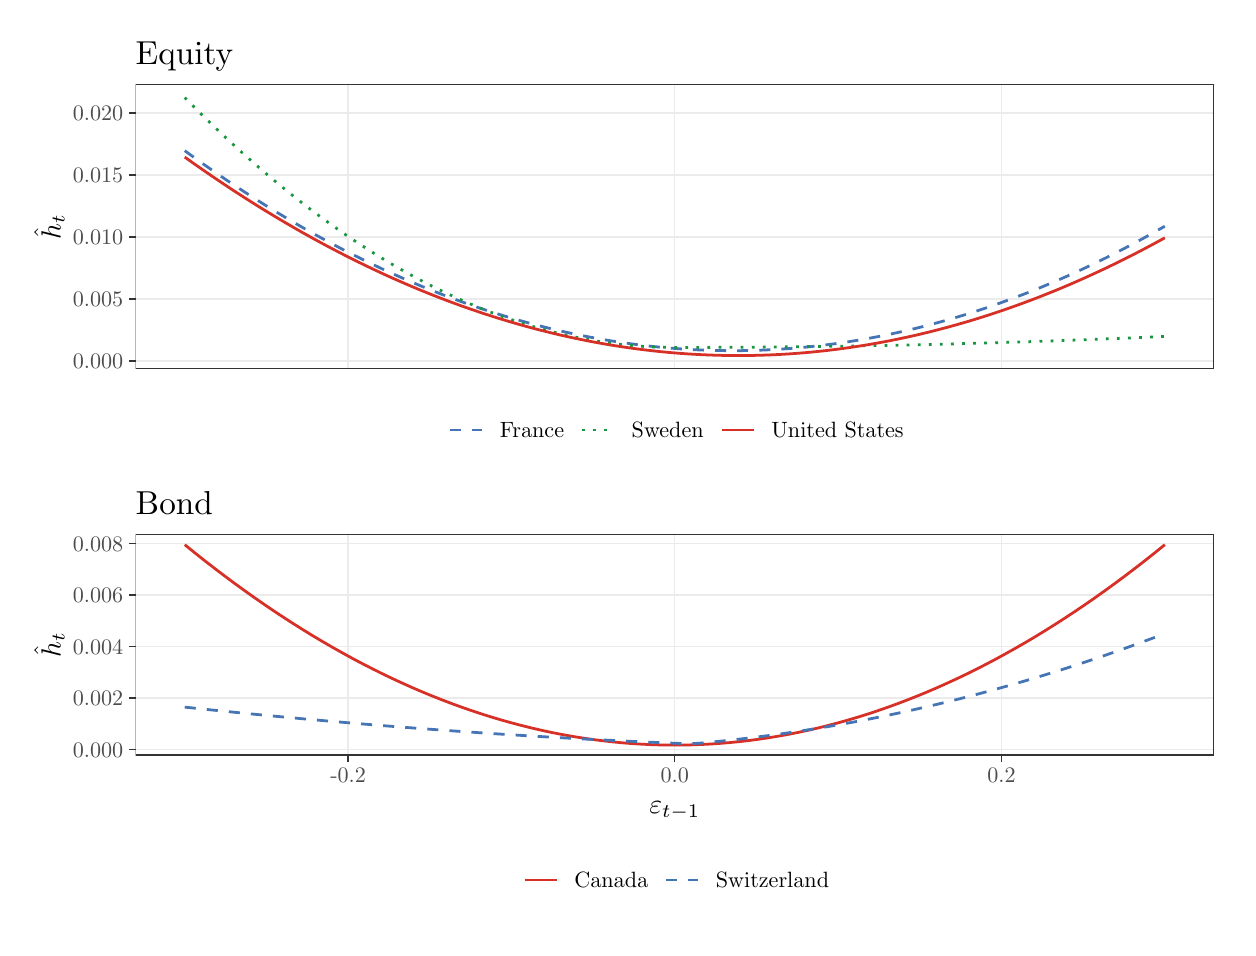
\begin{tikzpicture}[x=1pt,y=1pt]
\definecolor{fillColor}{RGB}{255,255,255}
\path[use as bounding box,fill=fillColor,fill opacity=0.00] (0,0) rectangle (433.62,325.21);
\begin{scope}
\path[clip] (  0.00,162.61) rectangle (433.62,325.21);
\definecolor{drawColor}{RGB}{255,255,255}
\definecolor{fillColor}{RGB}{255,255,255}

\path[draw=drawColor,line width= 0.5pt,line join=round,line cap=round,fill=fillColor] (  0.00,162.61) rectangle (433.62,325.22);
\end{scope}
\begin{scope}
\path[clip] ( 39.05,202.06) rectangle (428.62,304.62);
\definecolor{fillColor}{RGB}{255,255,255}

\path[fill=fillColor] ( 39.05,202.06) rectangle (428.62,304.62);
\definecolor{drawColor}{gray}{0.92}

\path[draw=drawColor,line width= 0.5pt,line join=round] ( 39.05,204.76) --
	(428.62,204.76);

\path[draw=drawColor,line width= 0.5pt,line join=round] ( 39.05,227.18) --
	(428.62,227.18);

\path[draw=drawColor,line width= 0.5pt,line join=round] ( 39.05,249.59) --
	(428.62,249.59);

\path[draw=drawColor,line width= 0.5pt,line join=round] ( 39.05,272.01) --
	(428.62,272.01);

\path[draw=drawColor,line width= 0.5pt,line join=round] ( 39.05,294.43) --
	(428.62,294.43);

\path[draw=drawColor,line width= 0.5pt,line join=round] (115.78,202.06) --
	(115.78,304.62);

\path[draw=drawColor,line width= 0.5pt,line join=round] (233.83,202.06) --
	(233.83,304.62);

\path[draw=drawColor,line width= 0.5pt,line join=round] (351.89,202.06) --
	(351.89,304.62);
\definecolor{drawColor}{RGB}{69,117,180}

\path[draw=drawColor,line width= 1.0pt,dash pattern=on 4pt off 4pt ,line join=round] ( 56.76,280.75) --
	( 60.33,278.16) --
	( 63.91,275.62) --
	( 67.49,273.13) --
	( 71.07,270.68) --
	( 74.64,268.28) --
	( 78.22,265.93) --
	( 81.80,263.63) --
	( 85.38,261.37) --
	( 88.95,259.16) --
	( 92.53,256.99) --
	( 96.11,254.88) --
	( 99.68,252.81) --
	(103.26,250.79) --
	(106.84,248.81) --
	(110.42,246.88) --
	(113.99,245.00) --
	(117.57,243.17) --
	(121.15,241.39) --
	(124.73,239.65) --
	(128.30,237.95) --
	(131.88,236.31) --
	(135.46,234.71) --
	(139.04,233.16) --
	(142.61,231.66) --
	(146.19,230.21) --
	(149.77,228.80) --
	(153.34,227.44) --
	(156.92,226.12) --
	(160.50,224.86) --
	(164.08,223.64) --
	(167.65,222.46) --
	(171.23,221.34) --
	(174.81,220.26) --
	(178.39,219.23) --
	(181.96,218.25) --
	(185.54,217.31) --
	(189.12,216.42) --
	(192.70,215.58) --
	(196.27,214.78) --
	(199.85,214.04) --
	(203.43,213.34) --
	(207.00,212.68) --
	(210.58,212.08) --
	(214.16,211.52) --
	(217.74,211.01) --
	(221.31,210.54) --
	(224.89,210.12) --
	(228.47,209.75) --
	(232.05,209.43) --
	(235.62,209.16) --
	(239.20,208.93) --
	(242.78,208.75) --
	(246.36,208.61) --
	(249.93,208.53) --
	(253.51,208.49) --
	(257.09,208.49) --
	(260.66,208.55) --
	(264.24,208.65) --
	(267.82,208.80) --
	(271.40,209.00) --
	(274.97,209.24) --
	(278.55,209.53) --
	(282.13,209.87) --
	(285.71,210.25) --
	(289.28,210.69) --
	(292.86,211.16) --
	(296.44,211.69) --
	(300.02,212.27) --
	(303.59,212.89) --
	(307.17,213.55) --
	(310.75,214.27) --
	(314.32,215.03) --
	(317.90,215.84) --
	(321.48,216.70) --
	(325.06,217.60) --
	(328.63,218.56) --
	(332.21,219.55) --
	(335.79,220.60) --
	(339.37,221.69) --
	(342.94,222.83) --
	(346.52,224.02) --
	(350.10,225.25) --
	(353.67,226.54) --
	(357.25,227.87) --
	(360.83,229.24) --
	(364.41,230.66) --
	(367.98,232.14) --
	(371.56,233.65) --
	(375.14,235.22) --
	(378.72,236.83) --
	(382.29,238.49) --
	(385.87,240.20) --
	(389.45,241.95) --
	(393.03,243.75) --
	(396.60,245.60) --
	(400.18,247.49) --
	(403.76,249.44) --
	(407.33,251.43) --
	(410.91,253.46);
\definecolor{drawColor}{RGB}{26,150,65}

\path[draw=drawColor,line width= 1.0pt,dash pattern=on 1pt off 3pt ,line join=round] ( 56.76,299.96) --
	( 60.33,296.34) --
	( 63.91,292.81) --
	( 67.49,289.34) --
	( 71.07,285.95) --
	( 74.64,282.64) --
	( 78.22,279.39) --
	( 81.80,276.22) --
	( 85.38,273.13) --
	( 88.95,270.11) --
	( 92.53,267.16) --
	( 96.11,264.28) --
	( 99.68,261.48) --
	(103.26,258.76) --
	(106.84,256.10) --
	(110.42,253.52) --
	(113.99,251.02) --
	(117.57,248.58) --
	(121.15,246.23) --
	(124.73,243.94) --
	(128.30,241.73) --
	(131.88,239.59) --
	(135.46,237.53) --
	(139.04,235.54) --
	(142.61,233.62) --
	(146.19,231.78) --
	(149.77,230.01) --
	(153.34,228.32) --
	(156.92,226.69) --
	(160.50,225.15) --
	(164.08,223.67) --
	(167.65,222.27) --
	(171.23,220.95) --
	(174.81,219.69) --
	(178.39,218.51) --
	(181.96,217.41) --
	(185.54,216.38) --
	(189.12,215.42) --
	(192.70,214.53) --
	(196.27,213.72) --
	(199.85,212.99) --
	(203.43,212.32) --
	(207.00,211.73) --
	(210.58,211.22) --
	(214.16,210.77) --
	(217.74,210.41) --
	(221.31,210.11) --
	(224.89,209.89) --
	(228.47,209.74) --
	(232.05,209.67) --
	(235.62,209.66) --
	(239.20,209.66) --
	(242.78,209.67) --
	(246.36,209.68) --
	(249.93,209.69) --
	(253.51,209.71) --
	(257.09,209.73) --
	(260.66,209.75) --
	(264.24,209.78) --
	(267.82,209.81) --
	(271.40,209.84) --
	(274.97,209.87) --
	(278.55,209.91) --
	(282.13,209.96) --
	(285.71,210.00) --
	(289.28,210.05) --
	(292.86,210.10) --
	(296.44,210.16) --
	(300.02,210.22) --
	(303.59,210.28) --
	(307.17,210.34) --
	(310.75,210.41) --
	(314.32,210.48) --
	(317.90,210.56) --
	(321.48,210.64) --
	(325.06,210.72) --
	(328.63,210.80) --
	(332.21,210.89) --
	(335.79,210.98) --
	(339.37,211.08) --
	(342.94,211.17) --
	(346.52,211.28) --
	(350.10,211.38) --
	(353.67,211.49) --
	(357.25,211.60) --
	(360.83,211.71) --
	(364.41,211.83) --
	(367.98,211.95) --
	(371.56,212.07) --
	(375.14,212.20) --
	(378.72,212.33) --
	(382.29,212.46) --
	(385.87,212.60) --
	(389.45,212.74) --
	(393.03,212.88) --
	(396.60,213.03) --
	(400.18,213.18) --
	(403.76,213.33) --
	(407.33,213.49) --
	(410.91,213.65);
\definecolor{drawColor}{RGB}{215,48,39}

\path[draw=drawColor,line width= 1.0pt,line join=round] ( 56.76,278.44) --
	( 60.33,275.90) --
	( 63.91,273.41) --
	( 67.49,270.96) --
	( 71.07,268.55) --
	( 74.64,266.19) --
	( 78.22,263.88) --
	( 81.80,261.61) --
	( 85.38,259.39) --
	( 88.95,257.22) --
	( 92.53,255.09) --
	( 96.11,253.01) --
	( 99.68,250.97) --
	(103.26,248.98) --
	(106.84,247.03) --
	(110.42,245.13) --
	(113.99,243.28) --
	(117.57,241.47) --
	(121.15,239.71) --
	(124.73,237.99) --
	(128.30,236.32) --
	(131.88,234.69) --
	(135.46,233.12) --
	(139.04,231.58) --
	(142.61,230.10) --
	(146.19,228.65) --
	(149.77,227.26) --
	(153.34,225.91) --
	(156.92,224.61) --
	(160.50,223.35) --
	(164.08,222.14) --
	(167.65,220.97) --
	(171.23,219.85) --
	(174.81,218.78) --
	(178.39,217.75) --
	(181.96,216.76) --
	(185.54,215.83) --
	(189.12,214.94) --
	(192.70,214.09) --
	(196.27,213.29) --
	(199.85,212.54) --
	(203.43,211.83) --
	(207.00,211.17) --
	(210.58,210.55) --
	(214.16,209.98) --
	(217.74,209.46) --
	(221.31,208.98) --
	(224.89,208.55) --
	(228.47,208.16) --
	(232.05,207.82) --
	(235.62,207.53) --
	(239.20,207.28) --
	(242.78,207.08) --
	(246.36,206.92) --
	(249.93,206.81) --
	(253.51,206.74) --
	(257.09,206.72) --
	(260.66,206.75) --
	(264.24,206.82) --
	(267.82,206.94) --
	(271.40,207.10) --
	(274.97,207.31) --
	(278.55,207.57) --
	(282.13,207.87) --
	(285.71,208.22) --
	(289.28,208.61) --
	(292.86,209.05) --
	(296.44,209.54) --
	(300.02,210.07) --
	(303.59,210.64) --
	(307.17,211.27) --
	(310.75,211.93) --
	(314.32,212.65) --
	(317.90,213.41) --
	(321.48,214.21) --
	(325.06,215.07) --
	(328.63,215.96) --
	(332.21,216.91) --
	(335.79,217.90) --
	(339.37,218.93) --
	(342.94,220.01) --
	(346.52,221.14) --
	(350.10,222.31) --
	(353.67,223.53) --
	(357.25,224.80) --
	(360.83,226.11) --
	(364.41,227.46) --
	(367.98,228.87) --
	(371.56,230.31) --
	(375.14,231.81) --
	(378.72,233.35) --
	(382.29,234.93) --
	(385.87,236.57) --
	(389.45,238.24) --
	(393.03,239.97) --
	(396.60,241.74) --
	(400.18,243.55) --
	(403.76,245.41) --
	(407.33,247.32) --
	(410.91,249.27);
\definecolor{drawColor}{gray}{0.20}

\path[draw=drawColor,line width= 0.5pt,line join=round,line cap=round] ( 39.05,202.06) rectangle (428.62,304.62);
\end{scope}
\begin{scope}
\path[clip] (  0.00,  0.00) rectangle (433.62,325.21);
\definecolor{drawColor}{gray}{0.30}

\node[text=drawColor,anchor=base east,inner sep=0pt, outer sep=0pt, scale=  0.80] at ( 34.55,202.00) {0.000};

\node[text=drawColor,anchor=base east,inner sep=0pt, outer sep=0pt, scale=  0.80] at ( 34.55,224.42) {0.005};

\node[text=drawColor,anchor=base east,inner sep=0pt, outer sep=0pt, scale=  0.80] at ( 34.55,246.84) {0.010};

\node[text=drawColor,anchor=base east,inner sep=0pt, outer sep=0pt, scale=  0.80] at ( 34.55,269.26) {0.015};

\node[text=drawColor,anchor=base east,inner sep=0pt, outer sep=0pt, scale=  0.80] at ( 34.55,291.67) {0.020};
\end{scope}
\begin{scope}
\path[clip] (  0.00,  0.00) rectangle (433.62,325.21);
\definecolor{drawColor}{gray}{0.20}

\path[draw=drawColor,line width= 0.5pt,line join=round] ( 36.55,204.76) --
	( 39.05,204.76);

\path[draw=drawColor,line width= 0.5pt,line join=round] ( 36.55,227.18) --
	( 39.05,227.18);

\path[draw=drawColor,line width= 0.5pt,line join=round] ( 36.55,249.59) --
	( 39.05,249.59);

\path[draw=drawColor,line width= 0.5pt,line join=round] ( 36.55,272.01) --
	( 39.05,272.01);

\path[draw=drawColor,line width= 0.5pt,line join=round] ( 36.55,294.43) --
	( 39.05,294.43);
\end{scope}
\begin{scope}
\path[clip] (  0.00,  0.00) rectangle (433.62,325.21);
\definecolor{drawColor}{RGB}{0,0,0}

\node[text=drawColor,rotate= 90.00,anchor=base,inner sep=0pt, outer sep=0pt, scale=  1.00] at ( 11.89,253.34) {$\hat{h}_t$};
\end{scope}
\begin{scope}
\path[clip] (  0.00,  0.00) rectangle (433.62,325.21);
\definecolor{fillColor}{RGB}{255,255,255}

\path[fill=fillColor] (146.13,167.61) rectangle (321.54,192.06);
\end{scope}
\begin{scope}
\path[clip] (  0.00,  0.00) rectangle (433.62,325.21);
\definecolor{fillColor}{RGB}{255,255,255}

\path[fill=fillColor] (151.13,172.61) rectangle (165.59,187.06);
\definecolor{drawColor}{RGB}{69,117,180}

\path[draw=drawColor,line width= 1.0pt,dash pattern=on 4pt off 4pt ,line join=round] (152.58,179.83) -- (164.14,179.83);
\end{scope}
\begin{scope}
\path[clip] (  0.00,  0.00) rectangle (433.62,325.21);
\definecolor{fillColor}{RGB}{255,255,255}

\path[fill=fillColor] (198.82,172.61) rectangle (213.28,187.06);
\definecolor{drawColor}{RGB}{26,150,65}

\path[draw=drawColor,line width= 1.0pt,dash pattern=on 1pt off 3pt ,line join=round] (200.27,179.83) -- (211.83,179.83);
\end{scope}
\begin{scope}
\path[clip] (  0.00,  0.00) rectangle (433.62,325.21);
\definecolor{fillColor}{RGB}{255,255,255}

\path[fill=fillColor] (249.27,172.61) rectangle (263.73,187.06);
\definecolor{drawColor}{RGB}{215,48,39}

\path[draw=drawColor,line width= 1.0pt,line join=round] (250.72,179.83) -- (262.28,179.83);
\end{scope}
\begin{scope}
\path[clip] (  0.00,  0.00) rectangle (433.62,325.21);
\definecolor{drawColor}{RGB}{0,0,0}

\node[text=drawColor,anchor=base west,inner sep=0pt, outer sep=0pt, scale=  0.80] at (170.59,177.08) {France};
\end{scope}
\begin{scope}
\path[clip] (  0.00,  0.00) rectangle (433.62,325.21);
\definecolor{drawColor}{RGB}{0,0,0}

\node[text=drawColor,anchor=base west,inner sep=0pt, outer sep=0pt, scale=  0.80] at (218.28,177.08) {Sweden};
\end{scope}
\begin{scope}
\path[clip] (  0.00,  0.00) rectangle (433.62,325.21);
\definecolor{drawColor}{RGB}{0,0,0}

\node[text=drawColor,anchor=base west,inner sep=0pt, outer sep=0pt, scale=  0.80] at (268.73,177.08) {United States};
\end{scope}
\begin{scope}
\path[clip] (  0.00,  0.00) rectangle (433.62,325.21);
\definecolor{drawColor}{RGB}{0,0,0}

\node[text=drawColor,anchor=base west,inner sep=0pt, outer sep=0pt, scale=  1.20] at ( 39.05,311.95) {Equity};
\end{scope}
\begin{scope}
\path[clip] (  0.00,  0.00) rectangle (433.62,162.61);
\definecolor{drawColor}{RGB}{255,255,255}
\definecolor{fillColor}{RGB}{255,255,255}

\path[draw=drawColor,line width= 0.5pt,line join=round,line cap=round,fill=fillColor] (  0.00, -0.00) rectangle (433.62,162.61);
\end{scope}
\begin{scope}
\path[clip] ( 39.05, 62.35) rectangle (428.62,142.01);
\definecolor{fillColor}{RGB}{255,255,255}

\path[fill=fillColor] ( 39.05, 62.35) rectangle (428.62,142.01);
\definecolor{drawColor}{gray}{0.92}

\path[draw=drawColor,line width= 0.5pt,line join=round] ( 39.05, 64.42) --
	(428.62, 64.42);

\path[draw=drawColor,line width= 0.5pt,line join=round] ( 39.05, 82.99) --
	(428.62, 82.99);

\path[draw=drawColor,line width= 0.5pt,line join=round] ( 39.05,101.57) --
	(428.62,101.57);

\path[draw=drawColor,line width= 0.5pt,line join=round] ( 39.05,120.15) --
	(428.62,120.15);

\path[draw=drawColor,line width= 0.5pt,line join=round] ( 39.05,138.72) --
	(428.62,138.72);

\path[draw=drawColor,line width= 0.5pt,line join=round] (115.78, 62.35) --
	(115.78,142.01);

\path[draw=drawColor,line width= 0.5pt,line join=round] (233.83, 62.35) --
	(233.83,142.01);

\path[draw=drawColor,line width= 0.5pt,line join=round] (351.89, 62.35) --
	(351.89,142.01);
\definecolor{drawColor}{RGB}{215,48,39}

\path[draw=drawColor,line width= 1.0pt,line join=round] ( 56.76,138.39) --
	( 60.33,135.49) --
	( 63.91,132.65) --
	( 67.49,129.88) --
	( 71.07,127.16) --
	( 74.64,124.50) --
	( 78.22,121.90) --
	( 81.80,119.35) --
	( 85.38,116.87) --
	( 88.95,114.45) --
	( 92.53,112.08) --
	( 96.11,109.78) --
	( 99.68,107.53) --
	(103.26,105.34) --
	(106.84,103.21) --
	(110.42,101.15) --
	(113.99, 99.14) --
	(117.57, 97.18) --
	(121.15, 95.29) --
	(124.73, 93.46) --
	(128.30, 91.69) --
	(131.88, 89.97) --
	(135.46, 88.32) --
	(139.04, 86.72) --
	(142.61, 85.18) --
	(146.19, 83.71) --
	(149.77, 82.29) --
	(153.34, 80.93) --
	(156.92, 79.63) --
	(160.50, 78.39) --
	(164.08, 77.20) --
	(167.65, 76.08) --
	(171.23, 75.02) --
	(174.81, 74.01) --
	(178.39, 73.07) --
	(181.96, 72.18) --
	(185.54, 71.35) --
	(189.12, 70.58) --
	(192.70, 69.87) --
	(196.27, 69.22) --
	(199.85, 68.63) --
	(203.43, 68.10) --
	(207.00, 67.63) --
	(210.58, 67.21) --
	(214.16, 66.86) --
	(217.74, 66.56) --
	(221.31, 66.33) --
	(224.89, 66.15) --
	(228.47, 66.03) --
	(232.05, 65.97) --
	(235.62, 65.97) --
	(239.20, 66.03) --
	(242.78, 66.15) --
	(246.36, 66.33) --
	(249.93, 66.56) --
	(253.51, 66.86) --
	(257.09, 67.21) --
	(260.66, 67.63) --
	(264.24, 68.10) --
	(267.82, 68.63) --
	(271.40, 69.22) --
	(274.97, 69.87) --
	(278.55, 70.58) --
	(282.13, 71.35) --
	(285.71, 72.18) --
	(289.28, 73.07) --
	(292.86, 74.01) --
	(296.44, 75.02) --
	(300.02, 76.08) --
	(303.59, 77.20) --
	(307.17, 78.39) --
	(310.75, 79.63) --
	(314.32, 80.93) --
	(317.90, 82.29) --
	(321.48, 83.71) --
	(325.06, 85.18) --
	(328.63, 86.72) --
	(332.21, 88.32) --
	(335.79, 89.97) --
	(339.37, 91.69) --
	(342.94, 93.46) --
	(346.52, 95.29) --
	(350.10, 97.18) --
	(353.67, 99.14) --
	(357.25,101.15) --
	(360.83,103.21) --
	(364.41,105.34) --
	(367.98,107.53) --
	(371.56,109.78) --
	(375.14,112.08) --
	(378.72,114.45) --
	(382.29,116.87) --
	(385.87,119.35) --
	(389.45,121.90) --
	(393.03,124.50) --
	(396.60,127.16) --
	(400.18,129.88) --
	(403.76,132.65) --
	(407.33,135.49) --
	(410.91,138.39);
\definecolor{drawColor}{RGB}{69,117,180}

\path[draw=drawColor,line width= 1.0pt,dash pattern=on 4pt off 4pt ,line join=round] ( 56.76, 79.69) --
	( 60.33, 79.31) --
	( 63.91, 78.93) --
	( 67.49, 78.56) --
	( 71.07, 78.20) --
	( 74.64, 77.84) --
	( 78.22, 77.48) --
	( 81.80, 77.13) --
	( 85.38, 76.79) --
	( 88.95, 76.44) --
	( 92.53, 76.11) --
	( 96.11, 75.78) --
	( 99.68, 75.45) --
	(103.26, 75.13) --
	(106.84, 74.81) --
	(110.42, 74.50) --
	(113.99, 74.19) --
	(117.57, 73.89) --
	(121.15, 73.59) --
	(124.73, 73.30) --
	(128.30, 73.01) --
	(131.88, 72.72) --
	(135.46, 72.45) --
	(139.04, 72.17) --
	(142.61, 71.90) --
	(146.19, 71.64) --
	(149.77, 71.38) --
	(153.34, 71.12) --
	(156.92, 70.87) --
	(160.50, 70.63) --
	(164.08, 70.38) --
	(167.65, 70.15) --
	(171.23, 69.92) --
	(174.81, 69.69) --
	(178.39, 69.47) --
	(181.96, 69.25) --
	(185.54, 69.04) --
	(189.12, 68.83) --
	(192.70, 68.63) --
	(196.27, 68.43) --
	(199.85, 68.24) --
	(203.43, 68.05) --
	(207.00, 67.87) --
	(210.58, 67.69) --
	(214.16, 67.51) --
	(217.74, 67.34) --
	(221.31, 67.18) --
	(224.89, 67.02) --
	(228.47, 66.86) --
	(232.05, 66.71) --
	(235.62, 66.57) --
	(239.20, 66.43) --
	(242.78, 66.66) --
	(246.36, 66.99) --
	(249.93, 67.34) --
	(253.51, 67.71) --
	(257.09, 68.11) --
	(260.66, 68.52) --
	(264.24, 68.96) --
	(267.82, 69.43) --
	(271.40, 69.91) --
	(274.97, 70.42) --
	(278.55, 70.95) --
	(282.13, 71.50) --
	(285.71, 72.07) --
	(289.28, 72.67) --
	(292.86, 73.29) --
	(296.44, 73.93) --
	(300.02, 74.59) --
	(303.59, 75.28) --
	(307.17, 75.99) --
	(310.75, 76.72) --
	(314.32, 77.47) --
	(317.90, 78.25) --
	(321.48, 79.05) --
	(325.06, 79.87) --
	(328.63, 80.71) --
	(332.21, 81.57) --
	(335.79, 82.46) --
	(339.37, 83.37) --
	(342.94, 84.30) --
	(346.52, 85.26) --
	(350.10, 86.24) --
	(353.67, 87.24) --
	(357.25, 88.26) --
	(360.83, 89.30) --
	(364.41, 90.37) --
	(367.98, 91.46) --
	(371.56, 92.57) --
	(375.14, 93.70) --
	(378.72, 94.86) --
	(382.29, 96.04) --
	(385.87, 97.24) --
	(389.45, 98.46) --
	(393.03, 99.71) --
	(396.60,100.97) --
	(400.18,102.26) --
	(403.76,103.58) --
	(407.33,104.91) --
	(410.91,106.27);
\definecolor{drawColor}{gray}{0.20}

\path[draw=drawColor,line width= 0.5pt,line join=round,line cap=round] ( 39.05, 62.35) rectangle (428.62,142.01);
\end{scope}
\begin{scope}
\path[clip] (  0.00,  0.00) rectangle (433.62,325.21);
\definecolor{drawColor}{gray}{0.30}

\node[text=drawColor,anchor=base east,inner sep=0pt, outer sep=0pt, scale=  0.80] at ( 34.55, 61.66) {0.000};

\node[text=drawColor,anchor=base east,inner sep=0pt, outer sep=0pt, scale=  0.80] at ( 34.55, 80.24) {0.002};

\node[text=drawColor,anchor=base east,inner sep=0pt, outer sep=0pt, scale=  0.80] at ( 34.55, 98.82) {0.004};

\node[text=drawColor,anchor=base east,inner sep=0pt, outer sep=0pt, scale=  0.80] at ( 34.55,117.39) {0.006};

\node[text=drawColor,anchor=base east,inner sep=0pt, outer sep=0pt, scale=  0.80] at ( 34.55,135.97) {0.008};
\end{scope}
\begin{scope}
\path[clip] (  0.00,  0.00) rectangle (433.62,325.21);
\definecolor{drawColor}{gray}{0.20}

\path[draw=drawColor,line width= 0.5pt,line join=round] ( 36.55, 64.42) --
	( 39.05, 64.42);

\path[draw=drawColor,line width= 0.5pt,line join=round] ( 36.55, 82.99) --
	( 39.05, 82.99);

\path[draw=drawColor,line width= 0.5pt,line join=round] ( 36.55,101.57) --
	( 39.05,101.57);

\path[draw=drawColor,line width= 0.5pt,line join=round] ( 36.55,120.15) --
	( 39.05,120.15);

\path[draw=drawColor,line width= 0.5pt,line join=round] ( 36.55,138.72) --
	( 39.05,138.72);
\end{scope}
\begin{scope}
\path[clip] (  0.00,  0.00) rectangle (433.62,325.21);
\definecolor{drawColor}{gray}{0.20}

\path[draw=drawColor,line width= 0.5pt,line join=round] (115.78, 59.85) --
	(115.78, 62.35);

\path[draw=drawColor,line width= 0.5pt,line join=round] (233.83, 59.85) --
	(233.83, 62.35);

\path[draw=drawColor,line width= 0.5pt,line join=round] (351.89, 59.85) --
	(351.89, 62.35);
\end{scope}
\begin{scope}
\path[clip] (  0.00,  0.00) rectangle (433.62,325.21);
\definecolor{drawColor}{gray}{0.30}

\node[text=drawColor,anchor=base,inner sep=0pt, outer sep=0pt, scale=  0.80] at (115.78, 52.34) {-0.2};

\node[text=drawColor,anchor=base,inner sep=0pt, outer sep=0pt, scale=  0.80] at (233.83, 52.34) {0.0};

\node[text=drawColor,anchor=base,inner sep=0pt, outer sep=0pt, scale=  0.80] at (351.89, 52.34) {0.2};
\end{scope}
\begin{scope}
\path[clip] (  0.00,  0.00) rectangle (433.62,325.21);
\definecolor{drawColor}{RGB}{0,0,0}

\node[text=drawColor,anchor=base,inner sep=0pt, outer sep=0pt, scale=  1.00] at (233.83, 41.40) {$\varepsilon_{t-1}$};
\end{scope}
\begin{scope}
\path[clip] (  0.00,  0.00) rectangle (433.62,325.21);
\definecolor{drawColor}{RGB}{0,0,0}

\node[text=drawColor,rotate= 90.00,anchor=base,inner sep=0pt, outer sep=0pt, scale=  1.00] at ( 11.89,102.18) {$\hat{h}_t$};
\end{scope}
\begin{scope}
\path[clip] (  0.00,  0.00) rectangle (433.62,325.21);
\definecolor{fillColor}{RGB}{255,255,255}

\path[fill=fillColor] (173.10,  5.00) rectangle (294.57, 29.45);
\end{scope}
\begin{scope}
\path[clip] (  0.00,  0.00) rectangle (433.62,325.21);
\definecolor{fillColor}{RGB}{255,255,255}

\path[fill=fillColor] (178.10, 10.00) rectangle (192.55, 24.45);
\definecolor{drawColor}{RGB}{215,48,39}

\path[draw=drawColor,line width= 1.0pt,line join=round] (179.55, 17.23) -- (191.11, 17.23);
\end{scope}
\begin{scope}
\path[clip] (  0.00,  0.00) rectangle (433.62,325.21);
\definecolor{fillColor}{RGB}{255,255,255}

\path[fill=fillColor] (229.21, 10.00) rectangle (243.67, 24.45);
\definecolor{drawColor}{RGB}{69,117,180}

\path[draw=drawColor,line width= 1.0pt,dash pattern=on 4pt off 4pt ,line join=round] (230.66, 17.23) -- (242.22, 17.23);
\end{scope}
\begin{scope}
\path[clip] (  0.00,  0.00) rectangle (433.62,325.21);
\definecolor{drawColor}{RGB}{0,0,0}

\node[text=drawColor,anchor=base west,inner sep=0pt, outer sep=0pt, scale=  0.80] at (197.55, 14.47) {Canada};
\end{scope}
\begin{scope}
\path[clip] (  0.00,  0.00) rectangle (433.62,325.21);
\definecolor{drawColor}{RGB}{0,0,0}

\node[text=drawColor,anchor=base west,inner sep=0pt, outer sep=0pt, scale=  0.80] at (248.67, 14.47) {Switzerland};
\end{scope}
\begin{scope}
\path[clip] (  0.00,  0.00) rectangle (433.62,325.21);
\definecolor{drawColor}{RGB}{0,0,0}

\node[text=drawColor,anchor=base west,inner sep=0pt, outer sep=0pt, scale=  1.20] at ( 39.05,149.34) {Bond};
\end{scope}
\end{tikzpicture}
